%=== Préambule ===========================================================

\documentclass{beamer}
\usepackage{pdfpages}
\usepackage[english]{babel}
\usepackage{xspace}
\usepackage{pifont}
\usepackage{hyperref}
\usepackage{listings}
\usepackage{csquotes}
\usepackage{graphicx}
\usepackage{animate,media9} %,movie15}
\usepackage{wrapfig}
\usepackage{pdfpages}
\usepackage{tikz}
\usepackage{natbib}
\uselanguage{English}
\usepackage{fontawesome5}
\languagepath{English}
\setcounter{tocdepth}{1}
\usepackage{setspace}
\usepackage{amsmath}
\def\glasses{{\sffamily 
\leavevmode\rlap{%
\rotatebox[origin=tr]{125}{J}\kern1ex%  
\rotatebox[origin=tr]{125}{J}}% 
\rotatebox[origin=c]{-90}{D}%   
\rotatebox[origin=c]{-90}{D}}%
\def\ialy{\sffamily 
\resizebox{1ex}{1.5ex}{\reflectbox{\rotatebox[origin=]{75}{J}}}\kern-1pt%
\rlap{\tiny$\ ^\bullet\kern2.5pt^\bullet$ }%
\rotatebox[origin=c]{-90}{D}%   
\rotatebox[origin=c]{-90}{D}\kern-1pt%  
\resizebox{1ex}{1.5ex}{\rotatebox[origin=]{75}{J}}}}


\lstset{
  numbers=left,
  basicstyle=\tiny\ttfamily,      
  breaklines=true, 
  showtabs=false,
  showstringspaces=false,
}  

%=== Configuration de Beamer et du thème metropolis ======================
\usepackage{bbding}
\usetheme[background=light]{metropolis}
\usepackage[clock]{ifsym}

\definecolor{mLightBrown}{HTML}{000000}
\definecolor{black}{HTML}{000000}
\setbeamercolor{structure}{fg=black,bg=mLightBrown}
\setbeamercolor{palette primary}{%
	use=normal text,
	fg=normal text.bg,
	bg=mLightBrown
}
%\setsansfont[BoldFont={Linux Libertine G Bold},Numbers={OldStyle}]{Linux Libertine G}

\metroset{block=fill}

%=== Page de titre =======================================================

%path to logo and biblio -> to be adapted to your local directories 
\newcommand\dirlogo{../../logos/}
\newcommand\dirbiblio{../../biblio}



\title{{\normalsize \vskip 2cm 
L'accès aux
métiers scientifiques pour les
étudiants en situation de handicap}}
\subtitle{\small T\'emoignage: Hugo S\'anchez-Reyes}
\author{Hugo S\'anchez-Reyes \\ {\tiny Charg\'e de Recherche, Institut de Recherche pour le Développement IRD - ISTerre} \\ 
\\
\\
\textit{Merci à : \hspace{15pt}

\includegraphics[height=1.3cm]{../../logos/IRD-OSUG-ALL.png}\\}
}


\date[2021]{\vskip -0.5cm \hfill 12 Janvier 2023}

\subject{Group Meeting}

\titlegraphic{\centering \vspace{-15pt}
\includegraphics[height=1.3cm]{../../logos/IRD-OSUG.png} \par} %\qquad  
\includegraphics[height=1.4cm]{../../logos/anr_eqtime.png} \par }


\addtobeamertemplate{frametitle}{}{%
\begin{tikzpicture}[remember picture,overlay]
  \node[anchor=north east,yshift=0.0ex] at (current page.north east) {
\includegraphics[height=4ex]{../../logos/IRD_neg}};
  %\node[anchor=north east,yshift=0.5ex] at (current page.north east) {\includegraphics[height=3.3ex]{\dirlogo/seiscope_color_light_background}};
\end{tikzpicture}}



%=== Document ============================================================

\begin{document}

% --- Préambule ---------------------------------------------------------------

\begin{frame}
 
\includegraphics[width=1.2\linewidth]{images/1st_slide_blur.png} 
\end{frame}


\begin{frame}
    \titlepage
\end{frame}


\section{Qui suis-je ?  }

\begin{frame}
 {Le handicap en France ... Parlons-en ! } 
 
 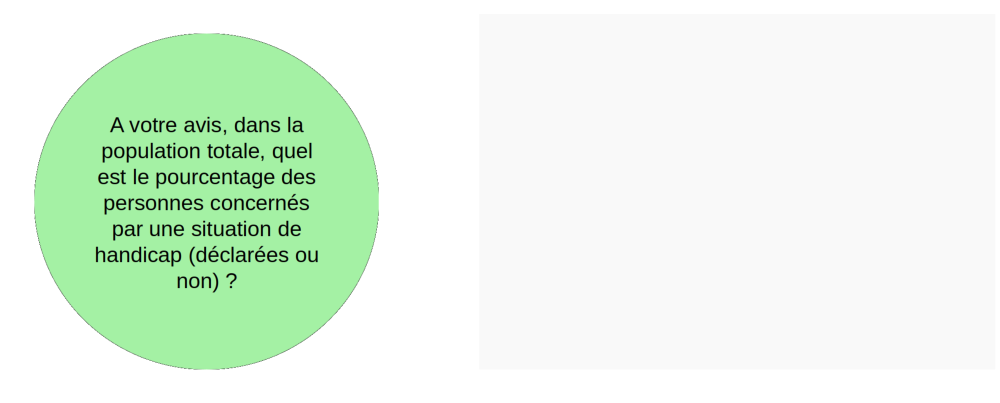
\includegraphics[width=1\linewidth]{images/handicap_cake0.png} 
 
\end{frame}

\begin{frame}
 {Le handicap en France ... Parlons-en ! } 
 
 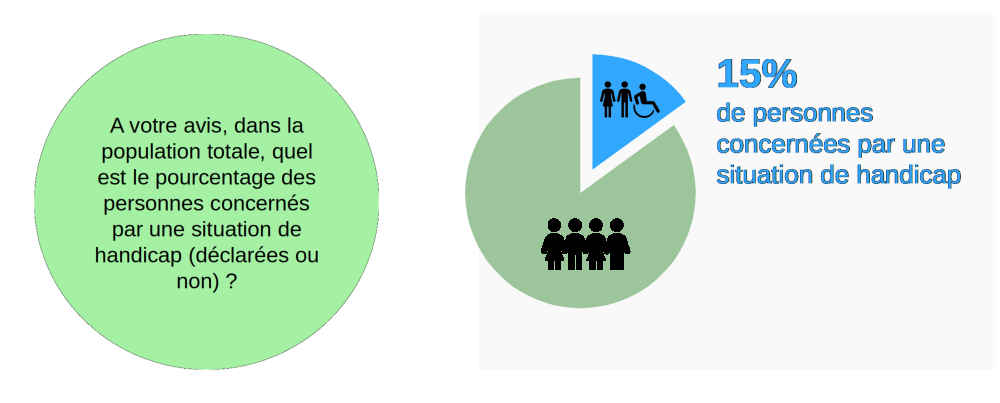
\includegraphics[width=1\linewidth]{images/handicap_cake1.png} 
 
\end{frame}


\begin{frame}
 {Le handicap en France ... Parlons-en ! } 
 
 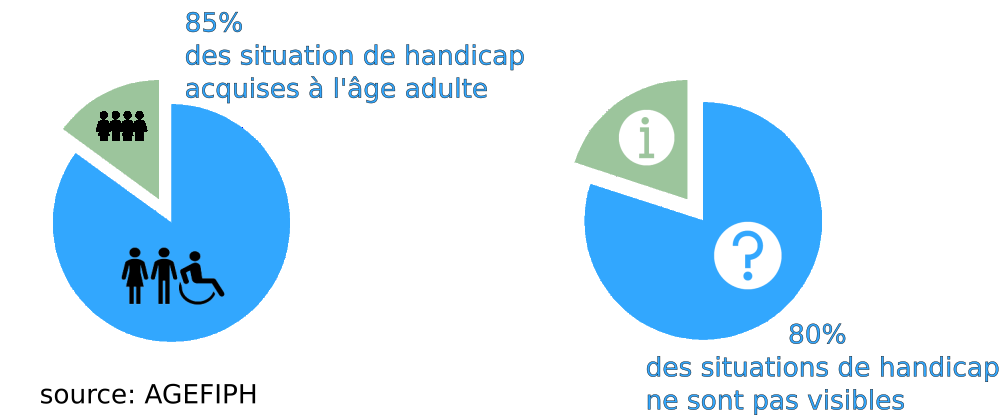
\includegraphics[width=1\linewidth]{images/handicap_cake2.png} 
 
\end{frame}



\begin{frame}
 {Le handicap en France ... et le handicap visuel } 

 \vskip -0.2cm \small Subdivision selon la famille de handicap \\
 \vskip 0.2cm
    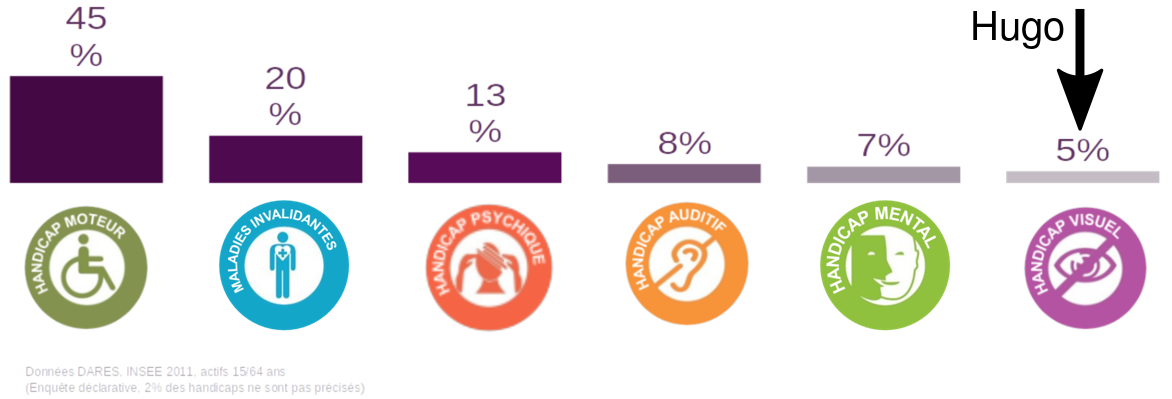
\includegraphics[width=1\linewidth]{images/handicaps.png} \\
\vskip -0.5cm Hugo : \pause
\vskip -0.2cm \begin{itemize}
% \item Mexicain d'origine \pause
 \item 33 ans \pause
 \item Handicap visuel - Diagnostique : \textbf{V}ogt-\textbf{K}oyanagi-\textbf{H}arada (VKH) \pause
 \item 28 ans d'être malvoyant (très experimenté) \pause 
 \item Pleines d'autres caractéristiques ... \pause 
 \item Mexicain d'origine, sismologue passionné, musicien, etc. \pause
\end{itemize}


 
\end{frame}

\begin{frame}
 
 \vskip -0.4cm \small Alors, comment je vois ? ... Si c'est une mauvaise journ\'ee, je vois comme ça  \vskip 0.1cm
 \centering 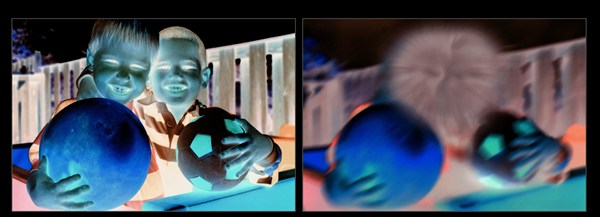
\includegraphics[width=0.75\linewidth]{images/visual_problem_neg.png}
 
\end{frame}



\section{Anectode acad\'emique}


\section{Parcours suivi}


\end{document}

